\documentclass[10pt]{ctexart}
\usepackage{listings}
\usepackage{amsmath} 
\usepackage{amssymb} 
\usepackage{xcolor}
\usepackage{xeCJK}
\usepackage{fontspec}
\usepackage{titlesec}
\usepackage{titletoc}
\usepackage{setspace}
\usepackage{graphicx}
\usepackage{geometry}
\usepackage[T1]{fontenc}  
\usepackage{textcomp}  
\usepackage{lmodern}
\usepackage[colorlinks,
            linkcolor=black,
            anchorcolor=black,
            citecolor=black]{hyperref}
\geometry{a4paper,scale=0.8}
\renewcommand\contentsname{Contents}
\setmonofont[Mapping={}]{Consolas} 
\setlength{\parindent}{0pt}
%\setmonofont[Mapping={}]{Consolas}    %英文引号之类的正常显示,相当于设置英文字体
%\setsansfont{Consolas} %设置英文字体 Monaco, Consolas,  Fantasque Sans Mono
%\setmainfont{Monaco} %设置英文字体
%\setmainfont{Helvetica Neue} %设置英文字体
% 定义可能使用到的颜色
%\setmainfont[BoldFont=SimHei]{SimSun}
\definecolor{CPPLight}  {HTML} {686868}
\definecolor{CPPSteel}  {HTML} {888888}
\definecolor{CPPDark}   {HTML} {262626}
\definecolor{CPPBlue}   {HTML} {4172A3}
\definecolor{CPPGreen}  {HTML} {487818}
\definecolor{CPPBrown}  {HTML} {A07040}
\definecolor{CPPRed}    {HTML} {AD4D3A}
\definecolor{CPPViolet} {HTML} {7040A0}
\definecolor{CPPGray}  {HTML} {B8B8B8}
\lstset{
    columns=fixed,       
    numbers=left,                                        % 在左侧显示行号
    frame=none,                                          % 不显示背景边框
    backgroundcolor=\color[RGB]{245,245,244},            % 设定背景颜色
    keywordstyle=\color[RGB]{40,40,255},                 % 设定关键字颜色
    numberstyle=\small\color{darkgray},                  % 设定行号格式
    commentstyle=\it\color[RGB]{0,96,96},                % 设置代码注释的格式
    stringstyle=\rmfamily\slshape\color[RGB]{128,0,0},   % 设置字符串格式
    showstringspaces=false,                              % 不显示字符串中的空格
    language=c++,                                        % 设置语言
    morekeywords={alignas,continute,friend,register,true,alignof,decltype,goto,
    reinterpret_cast,try,asm,defult,if,return,typedef,auto,delete,inline,short,
    typeid,bool,do,int,signed,typename,break,double,long,sizeof,union,case,
    dynamic_cast,mutable,static,unsigned,catch,else,namespace,static_assert,using,
    char,enum,new,static_cast,virtual,char16_t,char32_t,explict,noexcept,struct,
    void,export,nullptr,switch,volatile,class,extern,operator,template,wchar_t,
    const,false,private,this,while,constexpr,float,protected,thread_local,
    const_cast,for,public,throw,std},
    emph={map,set,multimap,multiset,unordered_map,unordered_set,
    unordered_multiset,unordered_multimap,vector,string,list,deque,
    array,stack,forwared_list,iostream,memory,shared_ptr,unique_ptr,
    random,bitset,ostream,istream,cout,cin,endl,move,default_random_engine,
    uniform_int_distribution,iterator,algorithm,functional,bing,numeric,},
    emphstyle=\color{CPPViolet},
    basicstyle=\linespread{1}\small\fontspec{Courier New Bold}\ttfamily,
    breaklines=true,
    %xleftmargin=1em,xrightmargin=1em, aboveskip=1em,
    % in the listings package configuration, try:  
    literate={"}{\textquotedbl}1,  
    tabsize=4, keepspaces=true
}
%\setmainfont{Courier New Bold}
%\begin{lstlisting}

%\end{lstlisting}
\CTEXoptions[today=old]
\title{TEMPLATE}
\author{}
\date{Last build at \today}

\begin{document}{
\begin{titlepage}
    \centering
    \vspace{2cm}
    {\scshape\Large South China University of Technology \par}
    \vspace{1cm}
    {\scshape\Large SCUT\_gugugu\par}
    \vspace{1.5cm}
    {\Huge\bfseries TEMPLATE\par}
    \vspace{4.5cm}
    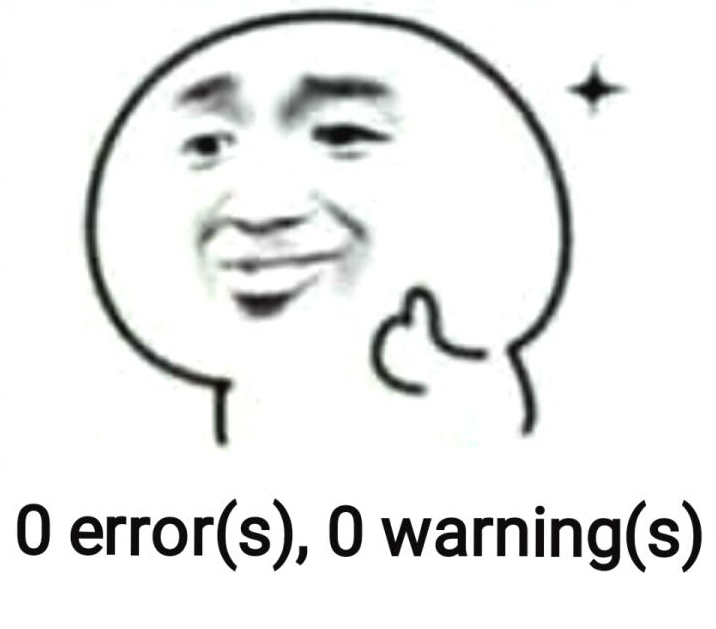
\includegraphics[width=0.5\textwidth]{./LOGO}\par\vspace{1cm}
    %\vspace{5cm}
    %{\Large\itshape Nickwzk\par}

    \vfill

% Bottom of the page
    {\large Last build at \today\par}

%\setcounter{page}{0}
\thispagestyle{empty}
%\newpage
\end{titlepage}
\tableofcontents
\newpage
\section{Graph Theory}
\subsection{Shortest Path}
尚未开始
\subsection{Network Flow}
修订稿 Created By ChrisJaunes

最大权闭合子图建模 eg: (+++) - (---) \\
定义:在一个有向图中,每个点都有一个点权。闭合子图:对于这个子图,它任意一个点的的后继必须在这个子图中。最大权闭合子图:在所有的闭合子图中,该图的点权和最大。\\
建模:\\
1. 建立超级源S和超级汇T\\
2. 把所有点权为正的点与S连接一条有向边,方向是从S到u,边权是点权;把所有点权为负的点与T连接一条有向边,方向是从u到T,边权是点权的相反数;\\
3. 原图中所有有向边的边权是INT\_MAX;也可以根据情况按照割的思想处理。\\ 
答案:最大权闭合子图的权值和就是所有点的点权和-该生成图的最小割\\
\\
独立集: 一个点集,点集中的各点没有关系。\\
最大独立集: 点的个数最多的独立集。 \\
求解一般无向图的最大团、最大独立集是NPC问题。\\
二分图最大独立集 = 点的总数 - 最小点覆盖。\\
最大点权独立集的点权和 = 所有点权和-最小点权覆盖的点权\\
路径覆盖:给定有向图 G=(V,E)。设 P 是 G 的一个简单路(顶点不相交)的集合。如果 V 中每个定点恰好在P的一条路上,则称 P 是 G 的一个路径覆盖。\\
最小路径覆盖:G 的最小路径覆盖是 G 所含路径条数最少的路径覆盖\\
建模:拆点,对于原图的(u,v),连接(u->v')\\
答案:原图的结点数-新图的最大匹配数\\
\\
最小割的可行边和必须边(所有割集的交集和并集) \\
注意:必须边⊆可行边.\\
1. 残余网络中有剩余流量的边一定不在最小割中\\
2. 残余网络中一条满流边的首尾还能相互到达,那么这条边不是可行边\\
3. 残余网络中一条满流的首尾分别与S和T在一个强连通分量中,那么这条边为必须边\\
具体实现,需要先跑最大流,然后Tarjan缩强连通分量,条件是:\\
可行边 : 两端不在一个强连通分量内。\\
必须边 : 一端在S的分量内,另一端在T的分量内。\\
必须边对于小规模也可以强行割去然后跑流判断流是否减少,暴力对费用流必须边同样适用\\
\\
求割边最少的最小割:把边的权值全部乘以一个较大的数E再加1, E要严格大于边的数量\\
最小割: ans/E;\\
最小割下的最小割边: ans \% E\\
公平分配模型:\\
题意:n个球队,已经有一些胜负场,现在还有一些场次,你去分配胜负,问每支球队有没有可能获胜\\
解:\\
1. 枚举每一个人,贪心计算比赛最大获胜次数max\_win\\
2. 将比赛当作节点,从源到比赛连比赛次数边\\
3. 分配比赛胜利者,从比赛到人连无穷边\\
4. 从人到汇连{max\_win - 已经获胜的比赛次数}的边\\
5. 检查是否能将比赛全部安排完\\
\\
混合图重定向为欧拉回路\\
1. 将所有的无向边随便定向,计算得到每个点的出度与入度之差deg\\
2. 建立源点汇点S,T\\
3. 对于deg>0的点v,连一条边S→u, 流为deg/2;\\
4. 对于deg<0的点u,连一条边u→T,流为-deg/2;\\
5. 对于有向边,忽略;对于无向边(u,v),连(u,v,1)\\
5. 判断是否能跑满流\\
\\
费用流:物品通过代价重复使用\\
1. 拆点,使用物品前和使用物品后\\
2. 对于节点[使用物品前]:考虑物品来源:源点{购买能力、购买费用}、节点[使用物品后]{INF、购买费用}; 去向:汇点{使用量、0}\\
3. 对于节点[使用物品后]:考虑物品来源:源点{使用量、0},去向:节点[使用物品前]\\
\\
费用流:物品通过代价延后销售\\
1. 拆点,生产物品和出售物品\\
2. 对于节点[生产物品]:考虑物品来源:源点{生产能力、 生产费用}; 去向: 节点[出售物品]{INF、保存的代价}\\
3. 对于节点[出售物品]:考虑物品来源:通过节点生产物品,去向:汇点{销售能力、销售费用}\\
\\
费用流:n个点m条带权有向边的图,要给边染色,染色的边形成若干个回路且每个点都恰好属于其中k个回路。问最少要染多少边权和的路。\\
一个回路里面各个点的入度=出度=1,各个点如果都恰好属于k个回路那么各个点的入度=出度=k。\\
这样就考虑用最小费用最大流了:\\
1. 所有点u拆成两点u和u',分别代表出度和入度\\
2. 原点向u连容量k费用0的边,u'向汇点连容量k费用0的边\\
3. 所有有向边<u,v>,u向v'连容量1费用边权的边\\
4. 这样跑最小费用最大流,如果最大流等于n*k,也就是说各个点的出度=入度=k,那么就有解,最小费用就是最小的解\\
\\
费用流:费用不是线性关系\\
费用为 $a * x^2$ : 拆边,拆成 a * 1, a * 3, a * 5, ...\\
费用为 之前的等待时间 + a : 反向考虑,倒数第i个点对整体贡献为 a * i, 拆点,拆成a, a*2, a*3, ...\\
\\
费用流:平面上给定一些黑点白点,要求一个黑点连接一个白点,并且所有线段都不相交\\
合法情况的连线,总长度明显比不合法情况的小, 题意可以转化为求让每条线段的长度和最小的方案\\
1、建立超级源超级汇\\
2、从超级源向左侧点连流量为1,费用为0的边\\
3、从左侧点向右侧点连流量为1,费用为两点欧几里得距离的边\\
4、从右侧点向超级汇连流量为1,费用为0的边\\
5、跑最小费用最大流\\
\\
区间k覆盖问题:给定n个带权开区间,区间最多可以选一次,要求保证实轴上的所有数被选择的次数要小于k次,问最大的权值。\\
1. 建立超级源超级汇\\
2. 源点向第一个点连一条容量为k、费用为0的边\\
3. 相邻节点连上用容量为k费用为0的边\\
4. 最后一个点向超级汇连一条容量为k、费用为0的边\\
5. 区间的两个端点之间连接一条容量为1的,费用为w的边\\
\\
区间至少ai覆盖问题\\
1. 建立超级源超级汇\\
2. 源点向第一个点连一条容量为INF、费用为0的边\\
3. 相邻节点连上用容量为INF-ai费用为0的边\\
4. 最后一个点向超级汇连一条容量为INF、费用为0的边\\
5. 区间的两个端点之间连接一条容量为INF的,费用为c的边\\
\\
分治优化建图\\
1. 费用为|ai-aj|可以利用差分性质通过累积权值之间的差值实现费用的绝对值\\
这样可以采用分治方式将边的数量从n*n将为n*logn\\
2. 一个点向一个区间的每一个点连边,可以利用线段树转为每个点最多向log个虚点连边\\
线段树上的点向孩子节点连边{INF},叶子节点向孩子连边{INF}
\subsection{Tree Related}
尚未开始
\subsection{LCA}
尚未开始
\subsection{Tarjan}
尚未开始
\subsection{Cactus}
尚未开始
\newpage
\section{Data Structures}
\subsection{Basic Structures}
尚未开始
\subsection{Heap Structures}
尚未开始
\subsection{Sequence Structures}
尚未开始
\subsection{Persistent Data Structures}
尚未开始
\subsection{Tree Structures}
尚未开始


\newpage
\section{String}
\subsection{Basics}
尚未开始
\subsection{String Matching}
尚未开始
\subsection{Suffix Related}
尚未开始
\subsection{Palindrome Related}
尚未开始


\newpage
\section{Math}
尚未开始


\newpage
\section{Geometry}
尚未开始


\newpage
\section{Game Theory}
\subsection{Bash's Game}
Bash's Game巴什博弈\\
有一堆个数为n的石子,游戏双方依次从中拿取,满足:\\
1.每次至少取1个,最多取m个.\\
最后取光者得胜。\\
结论: n = t(m+1) + r, 必败态:r = 0;\\
巴什博弈变种:\\
取一个指定集合的石头个数\\
取到最后一个石子输, n = t(m + 1)  + r, r = 1;\\
\subsection{Wythoff’s Game}
Wythoff’s Game(威佐夫博弈)\\
有两堆分别为(an, bn)的石子,游戏双方依次从中拿取,满足:\\
1.从任意一堆中取任意个 > 1。 
2.从两堆中取同样多个。
最后取完者胜.\\
结论: 对于任意的局势(a, b)(a < b),必败点为 (b-a)*(sqrt(5)+1)/2=a. \\
\subsection{Fibonacci’s Game / Zeckendorf's theory}
Fibonacci’s Game(斐波那契博弈)\\
有一堆个数为 n 的石子,游戏双方轮流取石子,满足:\\
1. 先手不能在第一次把所有的石子取完;\\
2. 之后每次可以取的石子数介于1到对手刚取的石子数的2倍之间(包含1和对手刚取的石子数的2倍)。\\
结论:必败点是斐波那契数\\
\par
齐肯多夫定理:任何正整数可以表示为若干个不连续的Fibonacci数之和\\
\subsection{Nim’s Game / Anti-Nim's Game / K-Nim's Game / Anti-K-Nim's Game}
Nim’s Game(尼姆博弈)\\
石子的个数可以等价成某个游戏的SG函数。\\
\par
有n堆石子,游戏双方依次从中拿取, 满足:\\
1.规定每次只能从一堆中取若干根, 可将一堆全取走,但不可不取.\\
最后取完者为胜。\\
结论:\\
T态:所有火柴数异或和为0\\
S态:所有火柴数异或和不为0\\
必胜态:S\\
\par
有n堆石子,游戏双方依次从中拿取,满足:\\
1.规定每次只能从一堆中取若干根, 可将一堆全取走,但不可不取.\\
最后取完者为败。\\
结论:\\
S0态:即仅有奇数个孤单堆\\
T0态:即仅有偶数个孤单堆\\
S1态:异或和大于0,且有1个充裕堆\\
T1态:不存在\\
S2态:异或和大于0,且有多个充裕堆\\
T2态:异或和等于0,且有多个充裕堆\\
必胜态:T0,S1,S2\\
必败态:S0,T2\\
\par
有n堆石子,游戏双方依次从中拿取, 满足:\\
1.规定每次只能至多k堆中取若干根, 可将k堆全取走,但不可不取.\\
最后取完者为胜。\\
结论:\\
对于每一堆,把它石子的个数用二进制表示\\
必败态:对所有的石子堆,如果在任何一个二进制位上1的个数总是k+1的整数倍\\
\par
有n堆石子,游戏双方依次从中拿取, 满足:\\
1.规定每次只能至多k堆中取若干根, 可将k堆全取走,但不可不取\\
最后取完者为败。\\
结论:\\
1.对于每一堆,把它石子的个数用二进制表示\\
2.所有的堆(非零堆,下同)全是1,此时如果1堆个数模k+1的结果是1则必败,否则必胜(我们可以通过 拿走0到k个堆来随意调整当前状态模的结果,然后再将所有大于1的堆降到1就行了)\\
3.有多于k个堆的个数大于1。必胜\\
\subsection{阶梯博弈}
有n个阶梯呈升序排列,每个阶梯上有若干个石子,游戏双方轮流取石子,满足:\\
1.将一个阶梯上的石子移任意个(>0)到前一个台阶。\\
当没有可行操作时(所有石子都被移动到了地面,即第0号台阶)输。\\
结论:\\
奇数号台阶的Nim游戏\\
变种1:
树上,每个石子只能往父亲节点移动.\\
变种2:\\
游戏双方在一个1*N的格子内挪动棋子,刚开始在若干个位置上有棋子,每个位置至多一个棋子\\
每一个选手可以进行的操作时选择一个棋子并把它向左方移动,当然不能越过其它的棋子,也不能超出边界。\\
谁不能移动谁就输了。求谁会赢?\\
结论:\\
将棋子位置按升序排列,然后从后往前两两绑成一对,如果个数是奇数,那么将第一个和边界外绑定.\\
一对棋子的前一个和前一对棋子的后一个之间有多少个空位置对最终的结果是没有影响的。\\
于是我们只需要考虑同一对的两个棋子之间有多少空位,将同一对棋子间的空位视为石子,做nim游戏\\
两对棋子间的空格数当奇数位石子,其他当偶数位石子,石子相右边移动\\
变种3:\\
山上有n个人,每个人给出距离山顶的距离,给出其中一个人为king,每次能挑选一个人向上移动,不能越过其他人,最后将king移动到山顶者获胜。问获胜者。\\
结论:\\
只要把King当作普通人一样处理即可。除了两种特殊情况:\\
1. 当King是第一个人时,Alice直接胜\\
2. 当King是第二个人且一共有奇数个人时,第一堆的大小需要减1。\\
\subsection{Multi-Nim}
有n堆石子,游戏双方依次从中拿取, 满足:\\
1.任意一堆石子中拿任意多个石子(不能不拿)\\
2.把一堆数量不少于2石子分为两堆不为空的石子\\
最后取完者为胜。\\
结论:\\
操作一与普通的Nim游戏等价\\
操作二实际上是将一个游戏分解为两个游戏,根据SG定理,我们可以通过异或运算把两个游戏连接到一起,作为一个后继状态\\
\begin{equation}
    SG(x)\equiv\left\{
    \begin{aligned}
    &x-1 & & (x mod 4 = 0) \\
    &x   & & (x mod 4 = 1 or 2)  \\
    &x+1 & & (x mod 4 = 3)
    \end{aligned}
    \right.
\end{equation}
\par
Multi-SG 游戏规定,在符合拓扑原则的前提下,一个单一游戏的后继可以为多个单一游戏。\\
Multi-SG其他规则与SG游戏相同。\\
注意在这里要分清楚后继与多个单一游戏\\
对于一个状态来说,不同的划分方法会产生多个不同的后继,而在一个后继中可能含有多个独立的游戏\\
一个后继状态的SG值即为后继状态中独立游戏的异或和\\
该状态的SG值即为后继状态的SG值中未出现过的最小值\\
\subsection{Every-SG}
给定一张无向图,上面有一些棋子,两个顶尖聪明的人在做游戏,每人每次必须将可以移动的棋子进行移动,不能移动的人\\
因为两个人都顶尖聪明,因此当一个人知道某一个游戏一定会输的话,它一定会尽力缩短游戏的时间,当它知道某一个游戏一定会赢的话,一定会尽力延长游戏的时间\\
对于还没有结束的单一游戏,游戏者必须对该游戏进行一步决策;\\
其他规则与普通SG游戏相同\\
Every-SG游戏与普通SG游戏最大的不同就是它多了一维时间\\
对于SG值为0的点,我们需要知道最少需要多少步才能走到结束\\
对于SG值不为0的点,我们需要知道最多需要多少步结束\\
这样我们用step变量来记录这个步数\\
\begin{equation}
    step(x)\equiv\left\{
    \begin{aligned}
    &0            & & u为终止状态 \\
    &max{step(v)} & & sg(u)!=0∧v为u的后继∧sg(v)=0\\
    &min{step(v)} & & sg(u)=0∧v为u的后继
    \end{aligned}
    \right.
\end{equation}
\subsection{树的删边游戏}
给出一个有 N个点的树,有一个点作为树的根节点。游戏者轮流从树中删去边,删去一条边后,不与根节点相连的部分将被移走。谁无法移动谁输。\\
结论:\\
Colon Principle:对于树上的某一个点,ta的分支可以转化成以这个点为根的一根竹子,这个竹子的长度就是ta各个分支的边的数量的异或和\\
叶子节点的SG值为0;中间节点的SG值为它的所有子节点的SG值加1后的异或和。\\

\subsection{Chomp's theory?}
取一个无关紧要的位置,如果对方必胜,则学习其策略,我方必胜.
\subsection{Other's theory?}
有n堆石子,游戏双方依次从中拿取, 满足:\\
1.规定每次能从任意多堆中取1根,不可不取.\\
最后取完者为胜。\\
结论:如果全是偶数,先手必败,否者先手必胜\\
\par
一个无相联通图,有一个点作为图的根。\\
游戏者轮流从图中删去边,删去一条边后,不与根节点相连的部分将被移走。\\
谁无路可走谁输。\\
结论:\\
Fusion Principle:环上的点可以融合,且不改变图的SG值,我们可以把一个带有奇数边的环等价成只有一个端点的一条边 而偶数边的环等价于一个点\\
\subsection{SG Theory}
\begin{lstlisting}
memset(mex, 0, sizeof mex);
for (int i = 1; i < maxN;++i) {
    for (int j = 1; j <= n;++j) {
        if (a[j] <= i)
            mex[SG[i - a[j]]] = i;
            for (int k = 1; i - k - a[j] > 0;++k)
                mex[SG[k] ^ SG[i - k - a[j]]] = 1;
    }
    for (int j = 0;; ++j)
        if (mex[j]!=i){
            SG[i] = j;
            break;
        }
}
\end{lstlisting}
\subsection{SJ Theory}
反公平游戏 Anti-SG Game\\
DAG上没有出度的点为胜利状态,其它定义与一般游戏相同。\\
现在的问题是解决多个反公平游戏的合并。\\
SJ定理说明:先手必胜,当且仅当以下两个条件同时成立或同时不成立:\\
1.合并的SG值为0;\\
2.所有游戏的SG值不超过1。\\
\subsection{Surreal Number Theory}


\newpage
\section{动态规划}
\subsection{最大子矩阵}
单调栈法:
\begin{lstlisting}
#include <bits/stdc++.h>
using namespace std;
const int MAXN = 1007;
int a[MAXN][MAXN], b[MAXN][MAXN];
pair<int, int> mp[MAXN * MAXN];
pair<int, int> off[MAXN][MAXN];
int tail;
pair<int, int> st[MAXN];
int Up[MAXN][MAXN];
int ans = 0;
void maintain(pair<int, int> v) {
    for(;tail && st[tail].first >= v.first; tail--) {
        ans = max(ans, st[tail].first * (v.second - st[tail-1].second-1));
    }
}
void clear(int pos) {
    for(;tail; tail--)
        ans = max(ans, st[tail].first * (pos -st[tail-1].second-1));
}
int main() {
    ios::sync_with_stdio(0); cin.tie(0);
    int n, m;
    cin >> n >> m;
    for(int i = 1; i <= n; i++)
        for(int j = 1; j <= m; j++) {
            cin >> a[i][j];
            mp[a[i][j]] = {i,j};
        }
    for(int i = 1; i <= n; i++)
        for(int j = 1; j <= m; j++) {
            cin >> b[i][j];
            off[i][j] = {i - mp[b[i][j]].first, j - mp[b[i][j]].second};

        }
    for(int i = 1; i <= n; i++) {
        st[0].second = 0;
        for(int j = 1; j <= m; j++) {
            Up[i][j] = i > 1 && off[i][j] == off[i-1][j] ? Up[i-1][j] + 1 : 1;
            if(j > 1 && off[i][j] == off[i][j-1]) 
                maintain({Up[i][j], j}); else {clear(j); st[0].second = j-1;}
            st[++tail] = {Up[i][j], j};
        }
        clear(m+1);
    }
    cout << ans << endl;
    return 0;
}
\end{lstlisting}
悬线法:
\begin{lstlisting}
#include <bits/stdc++.h>
using namespace std;
const int MAXN = 1007;
int a[MAXN][MAXN], b[MAXN][MAXN];
pair<int, int> mp[MAXN * MAXN];
pair<int, int> off[MAXN][MAXN];
int L[MAXN][MAXN], R[MAXN][MAXN], UP[MAXN][MAXN];
int main() {
    ios::sync_with_stdio(0); cin.tie(0);
    int n, m;
    cin >> n >> m;
    for(int i = 1; i <= n; i++)
        for(int j = 1; j <= m; j++) {
            cin >> a[i][j];
            mp[a[i][j]] = {i,j};
        }
    for(int i = 1; i <= n; i++)
        for(int j = 1; j <= m; j++) {
            cin >> b[i][j];
            off[i][j] = {i - mp[b[i][j]].first, j - mp[b[i][j]].second};
            L[i][j] = R[i][j] = j;
            UP[i][j] = 1;
        }
    for(int i = 1; i <= n; i++) 
        for(int j = 2; j <= m; j++) {
            if(off[i][j] == off[i][j-1]) L[i][j] = L[i][j-1];
        }
    for(int i = 1; i <= n; i++) 
        for(int j = m - 1; j >= 1; j--) {
            if(off[i][j] == off[i][j+1]) R[i][j] = R[i][j+1];
        }
    int ans = 0;
    for(int i = 1; i <= n; i++) 
        for(int j = 1; j <= m; j++) {
            if(i > 1 && off[i][j] == off[i-1][j]) {
                UP[i][j] = UP[i-1][j] + 1;
                L[i][j] = max(L[i][j], L[i-1][j]);
                R[i][j] = min(R[i][j], R[i-1][j]); 
            }
            ans = max(ans, (R[i][j] - L[i][j] + 1) * UP[i][j]);
        }
    cout << ans << endl;
    return 0;
}
\end{lstlisting}
\subsection{斜率优化}
\subsection{四边形不等式优化}
\subsection{忘情水二分}

\end{document}
